\section{Discussion and Background on Robustness}
\subsection{Morphogen Gradients and Developmental Robustness}

Given a morphogen distribution over one spatial dimension, one can determine how sensitive the thresholds of the target genes are to perturbations of the morphogen distribution.  This is discussed in Alon's text in chapter 8 "Robust Patterning in Development" \cite{designp}.  Here we will reproduce Alon's derivations for producing a morphogen profile ( distribution ) and his analysis of whether this profile is robust, but we will do so in the context of the morphogen Bicoid (Bc) and its robustness probe Hunchback (Hb), where similar analysis was done by Gregor and Houchmandzadeh \cite{pmid17632062}\cite{pmid11845210}.  Our analysis starts with a transport equation for the morphogen.
\begin{equation}\label{}
    \frac{\partial M}{\partial t} =  D \frac{\partial^2 M }{\partial x^2} - F(M)
\end{equation}
Here $F(M)$ is a function of the morphogen concentration and represents the degradation of the morphogen.  Notably missing from the equation is the production rate of the morphogen, as assumed from Gregor and in Alon's text the morphogen is assumed to be in steady state\cite{designp}.  Hence the time derivative is zero, and one can determine, or declare, the morphogen concentration by the boundary conditions:
$
    M(x = 0) = M_0 $ and $  M(x=\infty) = 0
$
 It is important to conceptually see what these conditions mean, since thermodynamic equilibrium in diffusion processes would lead to a morphogen distribution that is uniform over space, which we're about to see is not the case for our problem because a uniform profile occurs only if the system does not have sources and sinks.  Here we're assuming some source, a constant source such as ribosomes translating Bc mRNA at position x=0, and we are assuming a sink by the proteasome degradation of the Bc protein at $x=\infty$. \footnote[1]{ the idea that Bc mRNA is localized at x=0 was recently shown false, it was shown that Bc mRNA is also diffusing and closely follows the Bc protein profile, but for our discussion we'll assume that Bc is translated into protein at x=0 and then diffuses, and all of this is captured by our boundary condition.}
The Diffusion constant D determines the \textbf{absolute} length scale of the problem, which creates a problem for patterning mechanisms if the embryos have large variations in their size, since an intricate \textit{scaling} mechanism would be required, as diffusion is based on absolute length scales, this is discussed by Gregor and by Crocker \cite{pmid18328473}.  Assuming the variation of the embryos length is negligible we need to see how the scale of the problem is established. Alon's analysis starts with a linear degradation mechanism $F(M) =\alpha M $, where upon solving the PDE given the morphogen is in steady state, one arrives at:
\begin{equation}\label{ss}
    M(x) = M_0 e^{-\frac{x}{\lambda}}
\end{equation}

where $\lambda = \sqrt{\frac{D}{\alpha}}$, clearly when $x=\lambda$ the morphogen has reached a concentration of $\frac{M_0}{e}$, which is only about 33\% of its max, and after $2 \lambda$, the morphogen has reached a concentration of $\frac{M_0}{e^2}$ in general:
\begin{equation}\label{}
    x = \lambda, 2\lambda, .. n \lambda
\end{equation}
then
\begin{equation}\label{morpscale}
    M = \frac{M_0}{e},\frac{M_0}{e^2},..\frac{M_0}{e^n}
\end{equation}
 Using 'units' of $\lambda$ is not only useful for seeing how the morphogen decays as a function of absolute length, it is in fact the units the morphogen uses to create patterns, as when one anthropomorphizes the morphogen, they realize that the morphogen can not reproducible make patterns on any scale other than $ \lambda $, where reproducible means comparing the patterns \textbf{between} embryos.


  \subsection{Fine patterns}
   Let's see if the morphogen can create a fine pattern on the scale of $ 1 \mu m = $ when $ \lambda = 10 \mu m$. Now the morphogen creates the pattern by binding to the Hb promoter and stimulating Hb expression, so the Hb expression as a function of space is the pattern.  This is denoted by figure \ref{shift}.  In drosophila the x axis (the Anterior Posterior axis, major axis of the elliposdal embryo) is about 500 $\mu m$ and each nucleus is separated by about 10 $ \mu m$, since the pattern here is referring to the expression of Hb as a function of nuclear position, we see that $ 1 \mu m$ doesn't even make sense, since the smallest unit of our problem is $10 \mu m$,  So let's fix our ill-posed question to the morphogen trying to make a pattern over  $ 10 \mu m $ where $ \lambda =100 \mu m $.  Now to determine if a pattern can be created all we need to know is if the Hb promoter can detect (distinguish) Bc concentrations that are separated by $ 10 \mu m $  (two neighboring nuclei).  Well the answer is simple, \textbf{yes}, if we use the Hill model \eqref{segcon2hb}, to represent Hb's detection mechanism, then clearly the promoter can detect \textbf{any} concentration of Bicoid, and clearly any desired pattern could be produced  (To determine the pattern one simply defines a Bicoid concentration as the start of the pattern (i.e. a 'threshold concentration', $M(x)$) and and then inverts the Hill equation to find the Bc concentration and position, which come from equation \eqref{ss}).
 \begin{equation}\label{segcon2hb}
    \frac{[Hb]}{[Hb_{max}]} = \frac{1}{1 + e^{ -(w_{0} +  \left< n_{Bc} \right> w_{Bc}})}
\end{equation}

 But, we want to explore this problem from the perspective of robustness, that is if the Bc concentration deviates from its ideal profile for whatever reason (e.g. the mother laid less functional bc mRNA because only one of her bc alleles is functional (i.e. she is a heterozygote), or a slight variant of mRNA are laid in the oocyte etc. see for example\cite{pmid18687054} for a case of microscopy analysis of heterozygotes and homozygotes), then what would happen to our Hb profile.  In this sense, one may loosely say that we are interested in knowing if a nonrobust input can still be transformed into a robust output \footnote[2]{for thermodynamic modeling (fractional occupancy) this question is approximately answered by taking the derivative of the model $<N_{mRNA}>$ with respect to the input concentration that is varying, one will see that the effect is only at the border due to the form of the model}.

  A formal measure of this (robustness) is defined by Alon as the 'positional shift' that is by how many microns $\delta $ does our pattern shift.  To determine the function $\delta $ we need to perturb the production rate $M$ (i.e. the boundary condition at $x$ = 0) from $M$ to $M'$, then one can see $\delta $ from the graph in figure \ref{shift}.  When analyzing these equations, keep in mind that the Hb concentration is captured by the concentration of the morphogen $[M]$, so $M(x)$ and $M(x')$ represent the same Hb concentration.
  \begin{equation}\label{inverse}
    d x = \frac{d x }{d M} dM
  \end{equation}

\begin{equation}\label{solvex}
    dx = \delta = x - x'
  \end{equation}
  inverting equation \eqref{ss} we can isolate the position, hence solving for $x$:
  \begin{equation}\label{}
   x = \lambda \log{\frac{M}{M(x)}}
  \end{equation}
  now if we change the boundary condition to $M$', and solve for $x$', which represent the new border position of Hb expression:
  \begin{equation}\label{}
  x' = \lambda \log{\frac{M'}{M(x')}}
  \end{equation}
  now we have the pieces to calculate $\delta$,
  \begin{equation}\label{}
     \delta = \lambda \log{\frac{M}{M(x)} }- \lambda \log{\frac{M'}{M(x')}}
  \end{equation}
  since $M(x) = M(x')$, we arrive at:
  \begin{equation}\label{}
  \delta =  \lambda\log{\frac{M'}{M}}
  \end{equation}

\begin{figure},
  % Requires \usepackage{graphicx}
  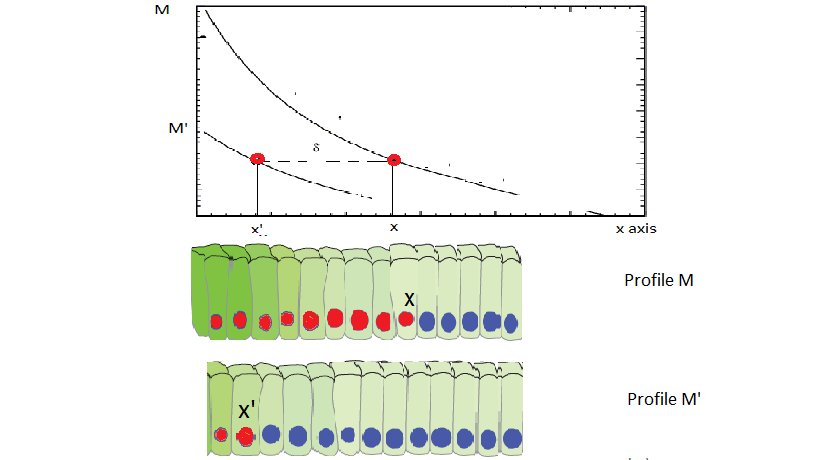
\includegraphics[width=1\textwidth]{sourcegraph}\\
  \caption{the green gradient represents the concentration of Bicoid and the orange nuclei denote Hb expression, while blue nuclei represent no Hb expression.  This figure was modified from figure 1 of \cite{pmid20066104}, and Alon's text\cite{designp}.}\label{shift}
\end{figure}

  Now that we know $\delta$ we can analyze why $\lambda$ is the effective length scale.  For example, let $M' = \frac{M}{2}$, then $\delta = \lambda log(\frac{1}{2}) \approx .7 \lambda $.  Recall, we wanted to find if the morphogen can create a pattern over $10 \mu m$, which was effectively the finest pattern since  $10 \mu m$ is the spacing between two cells or nuclei, but $.7 \lambda $ is a shift of 7 nuclei!  Clearly, for our problem, if the production rate varies by a 50\% reduction (as seen for classical heterozygote experiments,where one allele is lost), a precision on the order of the spacing between nuclei is not possible.


    Hence, the idea, of 'relevant length scale' for our problem can be understood from the perspective of what happens due to natural variations in morphogen gradient.

   % although other problems may have other reasons for defining their length scale (for example an optical wave moving through a lattice of atoms may compare the atomic spacing to the wavelength of the wave, where for wavelengths much shorter than the atomic spacing there may be no perturbations since the atoms 'see' both up and down fields, canceling any affects on the atoms movement.)\\
\par
Determining if a pattern is 'robust' to the morphogen's gradient (nearly independent of the morphogen's production rate) or if the pattern is 'fine-tuned' (extremely sensitive to any variation of the production rate) is an important problem in studying morphogen gradients - the parenthetical definitions both come from Alon's chapter 7 'Robustness of Protein Circuits'.

From our analysis, we see that the two goals of \textit{attaining} 'robust' outputs, while \textit{maintaining} a 'fine' pattern for the output are at odds with one another, there is a tradeoff.  The more robust we make our output to variations of the input then the less the module will be able to distinguish concentration differences of the input, and hence will not be able to produce a 'fine' pattern.  However, great attention has been given to 'combinatorial' regulatory mechanisms, in this sense one can imagine that noisy inputs do allow for robust and fine tuning, but the robustness is with respect to 'redundant' inputs \footnote[1]{For example, if two activators are both sufficient for transcription and both bind to the module that determines the output then random noise in one activator can clearly be compensated for by the other input}.  This can for example be achieved through cooperativity, or rather than robustness from combinatorial inputs, the promoter may have redundant binding sites for a key activator, thereby reaching the minimal number of morphogen to be bound for maximum expression.

For example Let us model the  border of rhomboid expression as a function of cooperativity.  Then we can ask how robust is the border with respect to variations of the concentrations of Tw and Dl \footnote[2]{Here we should be careful as Tw concentration is a function of Dl concentration, hence their noise is correlated, although less so at the dorsal border of the neuroectoderm, for simplicity we'll assume the noise in uncorrelated.}.

If we apply the analysis of Alon to the rhomboid gene\footnote[3]{Tissues can be defined by their gene expression, so our analysis is simply to find the threshold $T$, (the border concentration) of rhomboid.}, which is in this case activated by two morphogens $M_{dl}, M_{tw}$ we see that if we wish to apply 'thermodynamic modeling' it doesn't matter what the actual profiles of the Dl and Tw look like, all we need to do is vary these two concentrations simultaneously and analyze its effect on the model $<N_{mRNA}>$.  Using the fact that $ < ( \delta n_m )^2 > = \frac{\partial^2 \ln(\Xi)}{\partial n_m^2 }$, where $\Xi$ is the partition function for the CRM and morphogen system, one can check by simulation that $ < ( \delta n_m )^2 >= \sqrt{<n_m>}$, as shown from STAP simulations in figure\ref{rd}.\footnote{For example, I filtered Chip-chip data for the top 500 intensity peaks, further filtered to look at regions at least 100bp from the TSS of active genes, thereby excluding basal promoters with Dorsal bound to coactivators and Snail bound near the so-called 'pause button', which are unrepresentative of sequences of enhancers and would cause overfitting if included in the training set. To disentangle protein-DNA and protein-BTM interactions, the protein-DNA parameters were fit to Chip-chip data using the STAP program, where the data was filtered so as to only have verified chips for the protein, the protein-protein quenching interactions were also fit using filtered chip-chip data where all three proteins were jointly chipped in the same region, and the protein-protein coopertivity interactions were again fit using data where only twist and Dorsal were chipped but not snail.  Finally, the protein-BTM parameters were then determined using expression data from sequences that systematically explore the spacing of sites and hence exercise the various bins of the cooperativity and quenching functions (e g. the Ip and Szymanski data).  Then taking as subset of this data I predicted the Dorsal occupancy to determine the variance in the occupancy as a function of the occupation number in order to see if the process appeared Poisson, where the results are shown in figure \ref{rd}.}.  
For example, the Rhomboid expression at the dorsal border:
\begin{equation}\label{}
    <N_{rho} > = \frac{1}{1+e^{-<n_{dl}>w_{dl} + <n_{sn}>w_{sn} -<n_{tw}>w_{tw}}}
\end{equation}
the $w$'s are the parameters to be fit, and the $n$'s represent the average occupancy of each protein on the promoter.

\begin{figure}
   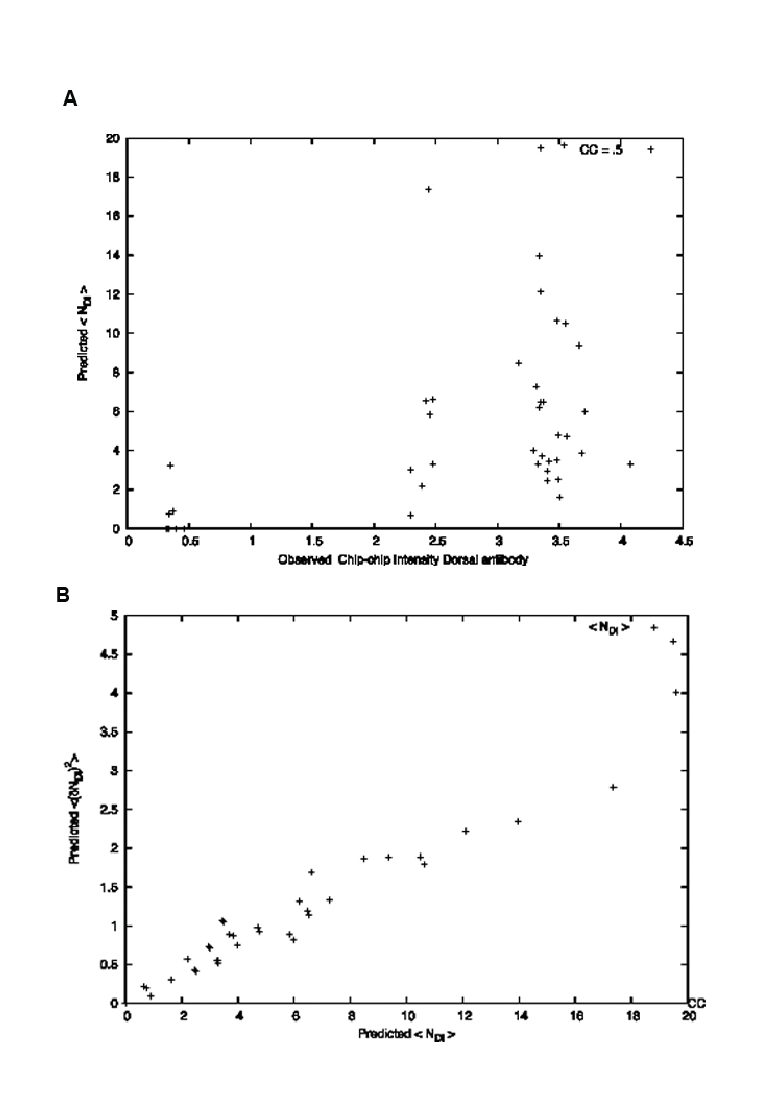
\includegraphics[]{dorsaltopvar}
   \caption{Panel A contains a scatter plot of predicted Dorsal occupancy vs subset of Dorsal Chip Intensities from MacArthur data\cite{pmid19627575}, where the Correlation Coefficient (CC) between the Intensities and the predicted occupancies was 0.5.  Panel B contains the variance as a function of the square root of the occupancy (the standard deviation of a Poisson process).}\label{rd}
\end{figure} 

It is known that twist alone is not sufficient for transcription, so we can set $w_{tw} = 0$, furthermore the dorsal border of rhomboid is well beyond snail's expression pattern, hence there will be no snail occupancy there, so $<n_{sn}>=0$.  Leaving:
\begin{equation}\label{}
    <N_{rho} > = \frac{1}{1+e^{-<n_{dl}>w_{dl} }}
\end{equation}
Therefore the variance in $<N_{rho} >$, which we'll label as $\sigma_{rho}$ will be roughly the range of expression:
\begin{equation}\label{}
 \sigma_{rho}  = \frac{1}{1+e^{-(<n_{dl}> +\delta n_m ) w_{dl} }} - \frac{1}{1+e^{-(<n_{dl}> -\delta n_m ) w_{dl} }}
\end{equation}
Once sigma is known one can then determine by how far the threshold concentration of Rhomboid ($M(x) = T$) has shifted in terms of cells, in the sense that $<N_{rho}^x > \pm \sigma_{rho}^x$ yields the two new expected values of Rhomboid, and one can simply compare these with the expected Rhomboid profile. (i.e.  $ <N_{rho}^x >- \sigma_{rho}^x  = <N_{rho}^{x'} >$  and $x-x' = \delta$ the shift.  Since $<n_{dl}>$ is related to the occupancy of twist, $<n_{tw}>$, this implies that the variance in dorsal occupancy $\delta n_{dl}$ captures how both dorsal and twist variations cause shifts in the dorsal border of rhomboid.  Another way is to simply look at that matrix element within the Hessian:
\begin{equation}\label{}
    \frac{\partial^2 <N_{rho}>}{\partial M_{tw} \partial M_{dl}}
\end{equation}
\subsection{Definition of Border and Production Rate}

Alon defines a transcription network as a set of nodes (target genes) and set of edges ( inputs to Hill function ).  The inputs to each each node are the three parameters that define the Hill function ( $n$, $K$ ,$\beta$ ), where $n$ is the Hill coefficient, $K$ is the equilibrium constant of the transcription factor activating or repressing the node \footnote[1]{ $\beta$ is the production rate ($V_{max}$) in Michelis Menten kinetics, that is maximum expression level}, and $\beta$ is the production rate of the gene.  Hence for a particular gene, which has mRNA concentration $Y$, one would have the following equation defining the gene's dynamics:
  \begin{equation}\label{}
    \frac{d Y}{d t} = \frac{\beta_{Y} }{ 1 + X/K} - \alpha
  \end{equation}
  Here $X$ is the concentration of an activator transcription factor and $K$ is the equilibrium constant for the the factor $X$ to its binding site, (for a repressor input simply inverse $X/K$), and $\alpha$ is the degradation rate of the mRNA or (protein product depending on what $Y$ represents).

  Clearly for any gene (node) $\beta$ is constrained by processtivity (the maximum translocation rate, $V_{max}$, of POLII along the gene, which is doubled with $10^{\circ}$ increase in temperature (ref Davidson), hence $\beta \in [0,V_{max}]$, furthermore since each gene, $g$,  will have its own production rate, we can say $\beta_g \in [0,\beta_{max}]$.

  Now from this description all of the information about the max production rate for our thermodynamic model (i.e. for a specific gene ) is encoded inside of the sigmoidal function of the $w$'s because the max production rate of the entire network is $\beta_{max}$, and because the model $<N>$ is divided by $\beta_{max}$ ( similar to Gregor's [Hb]/[Hbmax]) \footnote[1]{Sinha's lab noted that the correlation coefficient (one possible form of the objective function use to fit the parameters of the network) is scale invariant, hence they create a model where $\beta$ is a free parameter for EACH gene.  This is exactly the way Alon describes the network (where each gene gets its own $\beta$, however I prefer to not do that because that changes the meaning of the 'border', and hence the meaning of the $w$'s in the sigmoidal.}  This means the maximum expression, in our thermodynamic model is 1, and is at  $\alpha/ \beta_{max}$ (assuming steady state of mRNA expression).  Now as we vary the genes in the network, if we assume $\alpha$ is fixed, then for different steady state levels, it follows that $\beta$ must be varying (i.e. decreasing from $\beta_{max})$.  Hence there is a rule, which maps our sigmoidal function of the w's to $\beta$,  (the operation is not one to one due to saturation of the sigmoidal function, assuming we don't have infinite precision).

In our description of the profiles we have assumed that some profiles are not producing at $\beta_{max}$, that is we have lowered the level of gene expression because the level is lower then a reference gene which give $\beta_{max}$ (that is all genes whose expression level is at 1).

In assigning different expression levels ($\beta$), one is not affecting the \textbf{border} of the expression (i.e. the parameter $K$ ), as in this model the parameters ($\beta$ and $K$) are biochemically independent.  Hence some profiles which have their max expression levels below 1/2, do not have a border.  However, as pointed out by others, one could imagine a step wise (ladder) function, where there are multiple borders (i.e. the level =1 is not the max anymore).  For example we could assume an expression level of 2 as the max:
\begin{equation}\label{}
    f(Y_{ss}) = \beta_1\theta(K_1) + \beta_2\theta(K_2)
\end{equation}
Here $Y_{ss}$ is the steady state concentration, and $theta$ is the step function, hence once $X$ is above $K_1$, the level jumps to $\beta_1$, then it stays at that level until $X$ reaches $K_2$, at which point the level jumps to $\beta_1 + \beta_2$.  Actually this equation isn't properly written as one should start from the dynamic equation (with degradation) and solve, but the idea still holds, the borders are ($K_1$ and $K_2$), which allows for lower expressing modules to have a well defined border ($K$).

If we assume our set of target genes $\textbf{G}= {g_1,g_2,..g_n}$  (i.e. regulatory modules or sequences $\textbf{S}^{crm}$ in our Data set $\textbf{D}$), follow the production rate relation: $\beta_g \in (0,\beta_{max})$,  then using the Segal or Hill equation (equation \ref{segcon2},
 \begin{equation}\label{}
    <N_{g}> = \frac{1}{1 + exp{-(w_o +\sum_i<n_i>w_i)}}
 \end{equation}
 we can linearize it to solve for the w's:
 \begin{equation}\label{chi}
    \log{\frac{<N_{g_1}>}{1-<N_{g_1}>}} = w_o +\sum_i<n_i>w_i =\rm_{odds}
 \end{equation}

 if we assume the factors $i$ govern all $n$ genes then we have a matrix equation:
\[
\begin{pmatrix} \log{\frac{<N_{g_1}>}{1-<N_{g_1}>}}\\ \log{\frac{<N_{g_2}>}{1-<N_{g_2}>}} \\ \vdots \\  \log{\frac{<N_{g_n}>}{1-<N_{g_n}>}}\end{pmatrix}=
 \begin{pmatrix}
   1& <n_{X1}^{g_1}> & <n_{X2}^{g_1}> & <n_{X3}^{g_1}>  \\
   1&<n_{X1}^{g_2}> & <n_{X2}^{g_2}> & <n_{X3}^{g_2}> \\
    \vdots & \vdots & \vdots \\
   1&<n_{X1}^{g_n}> & <n_{X2}^{g_n}> & <n_{X3}^{g_n}>
 \end{pmatrix} \begin{pmatrix} w_0 \\ w_1 \\ w_2 \\ w_3 \end{pmatrix}
\]
Here we can use all (infinite if continuous) possible points along the profiles ($<N(z)>$ where $z$ is cellular position \footnote[1]{Recall that the occupancies are function of concentration: $<n_X> $, and hence are a function of position along the tissue.  If we have 40 cells that we measure $Y, X_1,X_2,X_3$, then and if we $n$ genes, then we'll have $n$*40 equations, and hence $n$*40 rows in our matrix.  Many of those equations will have the same value for $Y$, and hence can be set equal to each other, this is a consequence that there are many possible occupancies that lead to the same value of odds (Equation \ref{chi}), however if we fix the odds to be say 4,5,6,7 then we have a system of 4 equations, if we select one gene that has all these values reached at some point along its profile we'll have:
\[
\begin{pmatrix} 4 \\ 5 \\ 6 \\ 7\end{pmatrix}=
 \begin{pmatrix}
   1& <n_{X1(z1)}> & <n_{X2(z1)}> & <n_{X3(z1)}>  \\
   \vdots & \vdots & \vdots \\
1& <n_{X1(z4)}> & <n_{X2(z4)}> & <n_{X3(z4)}>
 \end{pmatrix} \begin{pmatrix} w_0 \\ w_1 \\ w_2 \\ w_3 \end{pmatrix}
\]
where $z$ is variable position along the profile, evaluated at 4 different positions, z1,.z4.  In this case it is reasonable and in fact mandatory that the occupancy change from one equation to another.  However, what if we collected 4 positions, that all had identical values of the odds?}

to solve for the w's, furthermore we also see that the points corresponding to $$<N_{g}> =\begin{cases}0  \\ 1 \end{cases}$$ lead to singularities, which is not surprising as there are infinite combinations of w's that in the limit give 0 or 1 for the sigmoidal function (another way to think of the 1,0 solutions, is that they have lost information, as there are multiple inputs that lead to 1 or 0, hence knowledge of these saturated outputs is uninformative of the exact input occupancy.).

However if $<N_{g}> \in (.1,.9)$, then our matrix equation is well defined.  (Here there may be multiple ways to to yield these solutions too, as are may ways to generate a fixed number from a sum of 3 integers). In particular if we collect all the genes that have a border (i.e.  $<N_{g}> = .5$, which is analogous to $X=K$ in the above discussion, and for our case it is like saying the gene's activator occupancy $<n>=K$) we then will have a subset of \textbf{G}, which yields a homogeneous system of equations:



\[
\begin{pmatrix} 0\\0\\ \vdots \\ 0\end{pmatrix}=
 \begin{pmatrix}
     1&<n_{X1}^{g_1}> & <n_{X2}^{g_1}> & <n_{X3}^{g_1}>  \\
   1&<n_{X1}^{g_2}> & <n_{X2}^{g_2}> & <n_{X3}^{g_2}> \\
    \vdots & \vdots & \vdots \\
   1&<n_{X1}^{g_m}> & <n_{X2}^{g_m}> & <n_{X3}^{g_m}>
 \end{pmatrix} \begin{pmatrix} w_0 \\ w_1 \\ w_2 \\ w_3 \end{pmatrix}
\]

Now if we imagine $m = 3$, we can make some important analysis (for $m > 3$, we can use least squares to solve $w$ \footnote[1]{ Least Squares gives an analytic solution to the minima, and this minima for a linear equation can be shown to be the global minima, for the situation with error in both inputs and outputs, I believe one finds that there are multiple roots and hence multiple minima, but the number of minima are small, hence one can exhaustively look at all the minima and simply find the smallest (the global)}).  If $m=3$, we have a system of 3 homogeneous equations, with 3 unknowns ($w$'s).  If our system is linearly independent, then the $w$'s must be zero, as that is the unique solution for a homogeneous system that is linearly independent ( if this is true for $m=3$, it obviously holds for $m >3$, which means adding more genes doesn't help us find nontrivial $w$'s, rather we must identify informative constructs (target genes) under particular conditions). 

Furthermore, if the variables are linearly independent for each gene (so we no longer have a system of equations for the $w$'s) then this indicates a method to see if the idea of putting multiple genes in the network (the system of equations) makes sense (i.e. does each gene have its own set of $w$'s, or are the $w$'s governing the entire network).  Adding more genes (which will increase $m$) will then cause the matrix equation to stay consistent or the system of equations will become inconsistent.  

Clearly the idea of 'Least Squares' already indicates the system of equations is inconsistent, and hence one is to maximize the projection (parallel component) of the vector Ax onto the data set y (a vector of odds), thereby minimizing the perpendicular component (i.e. the deviation ($\sum A_{ij} x_j - y_i$).  However, one could imagine creating a statistical test, like a t-test, where the average error component is the max of measurement and biological noise, then one can add a new gene to the matrix calculate the error and then could calculate, then one has a statistic which they can use to calculate the p value.

This is consistent with the idea of the network being completely governed by the occupancies.  This is basically telling us that there is only one typical target gene (that's why there is only one $w$ vector), and that that typical gene always expresses when the activator occupancy goes from $j$ to $j+1$ (this was an observation pointed out by W. Wedemeyer in a discussion on the pseudoinverse).

So if the factor's occupancies are linearly dependent\footnote[2]{ the $<n>$'s, I believe, would be linearly dependent because the idea that the occupancy goes from $j$ to $j+1$ for activation (when crossing the border), means there is an equation relating the occupancies, a constraint, namely $\sum_i<n_i>w_i = j+1$, where $j+1$ is playing the role of $K$}, then least squares will not work, as the design matrix, $A$, multiplied on its left by $A^T$ (i.e. $A^TA$) doesn't have an inverse if the factor's occupancies are linearly dependent (i.e. the design matrix is underdetermined), however, the method of svd allows for finding a best solution by using the pseudo inverse (this is also known as the Moore Penrose inverse).  Regardless, it is algebra, one inverts the/a matrix, which can be done by almost all linear algebra packages\footnote{In the case that $A^TA$ is zero determinant, we would like to still 'solve' for the $w$'s, or combinations of them, that our informative in a subspace of the parameter space (the $w$ space), this is the point of svd (singular value decomposition), which has been implemented by me in GSL for Chip-chip data as a component of a multiobjective function for occupancies and expression data (available at: https://github.com/jacobclifford/ConservedOccupancy, see the function compOccMat inside ExprPredictor.cpp file.} If we have $m >3$ and assume our system is undetermined, then we our left with finding a nontrivial solution in the null space (as we obviously don't want all the w's zero).  This means that there are infinite solutions to the w's (well, there would be only one normalized solution in the null space). 
\subsection{Uniform Shifts and Scale Invariance}

Scaling laws are relations between an attribute of a system and the size of the system (the size is the scale like length, mass, volume).
Power laws (e.g. polynomical equations relating the attribute to the size), are important in biology, because they indicate scale invariance.  That is the system is able to preserve the form of the relation as the scale varies.  In this sense scale invariance is a bit of a misnomer, it would have been better to say the equation is invariant, but such is tradition.
Work by Erives lab has shown that patterns are scale invariant (so the pattern width gets wider as the length of the embryo gets longer according to some law, possibly a power law).  This was achieved by looking at different sized eggs (different because they were different species of flies under different selection pressures).  Interestingly they noted the pattern's $cis$ regulatory module's grammar is NOT invariant.  That is the module changes (evolves by genetic mutations that eventually fix for adaptive sized embryos) to compensate for scaling.  Scaling laws are by nature very coarse grain, scaling laws do not tell one anything about the detailed mechanism within a object.  However, Erives work (or his student Crocker's work) in some sense linked the coarse with the fine details.
%
%For larger sized embryoes one can ask if the pattern has expanded, or if the absolute number of mrna has increased (presumably a consequence of expanded pattern),  if the nuclei are larger due to larger genomes etc.. then the expanded pattern may be isometric (pattern width divided by mass is a constant when one varies mass, hence the ratio is a constant, hence the relation w = km^a has 'a' equal to one, where w is width m is mrna (normally mass) 'a' is the allometric exponent, and k is the allometric constant. (ref answeres.com, wiki).  Isometry is the null hypothesis for scaling relations.
%
%If we have isometry for positional morphogens, then there are problems for explaining how the enhancers deal with such issues.  For example imagine one doubles the width of the embryo, than isometry predicts p = 2p'  where p' is the original pattern width, now if the number of nuclie are constant (2^14 ncs no matter what species) then presumably the the new width still occupies the same number of nuclei, the nuclei are just bigger or have a larger internuclear spacing ( 8 um for melanogaster at nc14, so maybe it just increases to 16um for a larger embryo).  If the time of development or some other mechanism does not occur than one could expect that the larger embryo would have less internuclear mRNA (cytoplasmic) since the absolute quantity would be the same..
%
%From wiki: " Isometric scaling occurs when changes in size (during growth or over evolutionary time) do not lead to changes in proportion."
%From wiki "size means dimensions such as length width height surface area, volume.
%the square-cuble law indicates that  an organism that doubles length will find its surface are quadruple, while volume and mass will increas by a factor of eight!"  This is interesting for maternal genes, do they increase 8 fold when length increases?, something increase 8 fold what is it?
%
%One would expect that their is negative allometry for rho expression since, the number of cis-elements is fixed (and therefore show negative allometry), hence the only way to get back to isometry for an expanded pattern is for the promoter to fire at a stronger rate, or for the nc time to change allowing for more steady state tf-crm interaction, that's important to change up the time since the spatial averaging is affected by the increased internuclear distances nuclear distances.  I think i read the the development is longer for larger embryoes (find ref).  This is an important relation the one of scale invariance being related to time, it may be that the transformation for invariance must not only be kx, but also kt, that is when scale changes so does the time scale.  cr. maxwell equations, scale invariance.
%
%scaling is essentially, using different units, if x -> 100*x, that's like saying we'll plug in our function cm instead of m, so all of our measurements have to be scalled by 100, since there are 100 cm per meter.
%
%the amount of scaling refers  to the alometric exponent, and it should be noted that power laws (polynomial equations as above, or distributions with a long tail) and exponentail exp(kx), both exhibit skaling since f(kx) proportional to f(x), as:
%$exp(k5x) = f(5x) = f(x)^5, actually this system does not exhibit scaling. but f(5x) = k(5x)^a = 5^a*f(x)$ which is proportional to the original, meaning the shape of the function stays fixed.  Note, gaussians, do not exhibit this bahavior, therefore the shape changes when the scale changes, that is, gaussians are not scale invariant: (figure:  gausScale), unless the width or shape parameter sigma is heteroscadastic over all scales, then a change in units, will cause a corresponding change in sigma, actually since the factor x/s is unitless it automatically is scale invariant!  Actually the problem is one like Maxwell's equations, the function is a two parameter or two dimensional function, with respect to x and s..  just as maxwells requires x -> ax, and t -> at.
%
%another problem of scaling is that for larger embryos with absolute quantities of bicoid constant, this doesn't make sense for Dorsal, as larger embryoes will require larger genomes that require larger nuclei the larger nucle in turn will require more activated toll receptors on the vitellane membrane, which means more spatzle will be required, in order to activate all of these receptors.  Now an increase in devo time, and especially sampling time of the genome, may compensate these factors.
%two problems, there are conflicting lines of evidence of that there are actually more nuclei in larger embryos, and that the devo times are the same.  This is same old bus from bio, one states knowledge as if its truth (since they're an authority) but in reality (in quantitative) they don't know what their talking about.
%
%heterochrony an idea of ernest hackel in 1890 mentioned that changes in rates can effect development, leading to changes in size and shape. pedomorphosis is the retention in adults of juvenile phenotypes, where the juvenile phenotypes can readily be adapted to change, while specialized adult features are resistant to change.  neoteny is also the retention of juvenile in the mature.
%////
%Scaling:  Direct quotes, and paraphrasing from the following:
%"Diffusion and scaling during early embryonic pattern formation", 2005, Gregor
%Using diffusion equation one sees that the length scale leads to nonscaling behavior, that is once the solution is solved the relavant constants are not dependent on the scale of the system, the constants, like the decay term in exp(-xt) the decay term 't', this constant is Dt' , which is the diffusion constant and the lifetime of morphogen.  If neither the lifetime nor the diffusion constant depend on the length scale of the system, then clearly the system will have no way to scale the gradient when the overall system (egg length) changes size.
%"Scaling of Gene expression profiles" page 18405, "Diffusion-based models provide no natural mechanism for generating spatial patterns that scale with size of the egg."  "the diffusion and biochem reactions, the diffusion constant and reaction rates determine an absolute length scale., thus when the size of the system changes, the spacing of the pattern elements would remain fixed"
%
%Mechanisms for scaling (page 1405 section "Scaling of gene expression profiles")
%two mechanisms for generating scaled versions of these profiles in species with larger embryos:
%1. the Bcd gradient could stay the same, and the cis-acting control sites of downstream genes could have adapted over evolution so that specific genes are activated by lower concentration of Bcd in species with larger eggs.
%2. (the alternative hypothesis), the Bcd gradient itself could scale, while the readout mechanisms encoded in the control sites of downstream genes are conserved across species".
%scaling is essentially, using different units, if x -> 100*x, that's like saying we'll plug in our function cm instead of m, so all of our measurements have to be scalled by 100, since there are 100 cm per meter.
%
%To distinguish the possibilities, they examined Bcd protein profiles from stained immunofluorescently, in L sericata, D mel,
%they noted Houchmandzadeh 2002, to show that the considerable  variability within one species jived with Houchmandzadeh's results! (last sentence page 18405 and figure 3A).
%
%Conclusion for how scaling of Bic gradient achieved: lambda = Dt, and of these two options, D is changed by 'effective transport parameter b', or t is changed by varying degradation machinery or someother species specific lifetime  adaptation.
%
%" of the many possible mechanisms for scaling, the only one taht is consistent with our data is variation in the effective lifetime of the Bcd protein itself."
\subsection{Molecular basis for Robustness of Morphogen gradients}

%Seeing that the linear degradation term in the morphogen PDE did not lead to a robust solution, a different functional form is needed for degradation, (assuming the Diffusion Coefficient and
Alon and Eldar's work show that a robust profile would require a degradation rate that is a nonlinear implicit function of space, $F(M) = -kM^2$, a power law for the degradation is worked out in Eldar's paper that shows robustness\cite{pmid12239569}.  Furthermore Gregor showed that among different Dipterian species that have different sized embryos the domain on the Bicoid protein that is targeted for degradation has been fine tuned by evolutionary mutations thereby allowing for a scaling mechanism between the different sized embryos that leads to a robust profile for Bicoid.  Gregor also analyzed the possibilty that target gene's cis regulatory modules may be fine tuning the Bicoid binding sites to achieve a mechanism to scale the patterns in larger embryos\cite{pmid16352710}\cite{pmid16352710}.  Crocker analyzed cis regulatory modules of Dorsal and Twist targets and found that the spacing between Twist and Dorsal binding sites had varied, by testing the effects of this variation in a \textit{in vivo} study they showed that changing the spacing (the number of base pairs between Dorsal and Twist sites) changed the target profile's anatomical positional border (the neuroectoderm- dorsal ectoderm border of the embryo), hence explaining the scaling mechanism for different sized embryos by the architecture of the enhancer.\footnote[1]{Crocker's assumptions assume same number of nuclei at nc14 = $2^{14} \simeq 16000$, however there has been indications that the number of nuclei scale with size of embryo, indicating nuclear cycles may not be completey synchronized, or there are more maternal nuclei in the syncitium (the chamber that holds the egg) than the initial mother's egg (haploid nucleus).\cite{kreitman} seeing that there is variation in the number of nuclei, that indicates that for target genes making decisions at nc9, then by nc14 the width, $w$, of the expression pattern will not minimally be $w \approx \sqrt{\frac{2^{14}}{2^9}} =5 $ nuclei as indicated by Bialek in his response to Sven Bergman's paper on pre-steady state decoding\cite{Response}\cite{pmid17298180}. } 